\documentclass[fleqn]{article}

\usepackage{graphicx}
\usepackage{xurl}
\usepackage{url}
\usepackage{caption}
\usepackage{fancyhdr}
\usepackage{mathtools}
\usepackage{amsmath}
\usepackage{amssymb}
\usepackage{tikz}
\usepackage{listings}
\usepackage{xcolor}
\usepackage{float}

\definecolor{codegreen}{rgb}{0,0.6,0}
\definecolor{codegray}{rgb}{0.5,0.5,0.5}
\definecolor{codepurple}{rgb}{0.58,0,0.82}
\definecolor{backcolour}{rgb}{0.95,0.95,0.92}

\lstdefinestyle{mystyle}{
	backgroundcolor=\color{backcolour},   
	commentstyle=\color{codegreen},
	keywordstyle=\color{magenta},
	numberstyle=\tiny\color{codegray},
	stringstyle=\color{codepurple},
	basicstyle=\ttfamily\footnotesize,
	breakatwhitespace=false,         
	breaklines=true,                 
	captionpos=b,                    
	keepspaces=true,                 
	numbers=left,                    
	numbersep=5pt,                  
	showspaces=false,                
	showstringspaces=false,
	showtabs=false,                  
	tabsize=2
}

\lstset{style=mystyle}

\usepackage{xepersian}

\settextfont[BoldFont={XB Zar bold.ttf}]{XB Zar.ttf}
\setlength\parindent{0pt}

\title{

\includegraphics[width=0.4\textwidth]{sharif.png}\\
\normalsize{دانشکده مهندسی کامپیوتر}\\
\vspace{1cm}
	
\huge{آزمایشگاه طراحی سیستم‌های دیجیتال}
\\
\Large{گزارش آزمایش هفتم}
\\
}

\author{
\\
دکتر سیاوش بیات سرمدی
\\
\\
پارسا محمدیان --- 98102284
}

\date{\today}

\begin{document}

\clearpage\maketitle
\thispagestyle{empty}

\newpage

\pagestyle{fancy}
\lhead{آزمایشگاه طراحی سیستم‌های دیجیتال}

\rhead{پارسا محمدیان}


\tableofcontents

\setcounter{page}{1}

\newpage

\section{مقدمه}

\subsection*{عنوان گزارش}
\lr{ALU} اعداد مختلط
\subsection*{موضوع}
استفاده از نرم‌افزارهای طراحی به کمک کامپیوتر \footnote{\lr{CAD}} برای طراحی 
و پیاده‌سازی مدار پشته به صورت توصیف رفتاری.
\subsection*{شرح ابزارها و برنامه‌های مورد استفاده}
در این آزمایش از نرم‌افزار \lr{ISE Desgin Suite} که محصول شرکت \lr{Xilinx} است 
استفاده کرده‌ام.

\section{چارچوب نظری و شرح آزمایش}
ابتدا ماژول‌های مورد نیاز را طراحی می‌کنیم. 

ماژول جمع و تفریق کننده در فایل 
\lr{complex\_adder\_subtractor.v} 
قرار دارد. برای جمع اعداد مختلط بخش موهومی با موهومی و بخش حقیقی با حقیقی جمع می‌شود. در تفریق نیز 
همین کار متناظرا انجام می‌شود. 

ماژول ضرب کننده در فایل 
\lr{complex\_multiplier.v} 
موجود است. ضرب کردن دو عدد مختلط مانند ضرب کردن دو عبارت دو جمله‌ای است و این رابطه به صورت رفتاری توصیف شده است.

نوبت به ماژول حافظه می‌رسد. پیاده سازی حافظه در فایل 
\lr{ram.v} 
موجود است.

در آخر در فایل 
\lr{cpu.v} 
ماژولی برای خواندن دستورات از حافظه و اجرای آنان را طراحی می‌کنیم. این پردازنده از نوع پشته‌ای است. جزئیات کارکرد این 
پردازنده به صورت کامنت در کنار پیاده‌سازی آمده است.

\section{تست مدار}
برای تست هر ماژول یک فایل تست بنچ برای آن می‌نویسیم.

فایل‌های تست به ترتیب 
\lr{tb\_complex\_adder\_subtractor.v} 
و 
\lr{tb\_complex\_multiplier.v} 
و 
\lr{tb\_ram.v} 
می‌باشند. در آخر یک فایل 
\lr{computer.v} 
برای کنار هم قرار دادن قطعات نوشته شده است که به نوعی تست 
\lr{cpu} 
است.

از آنجایی که ماژول‌های 
\lr{computer} 
و 
\lr{cpu} 
کمی پیچیده هستند، اجرای آن را توضیح می‌دهم. در ماژول کامپیوتر، پردازنده و رم قرار گرفته است. برای 
اینکه بتوانیم برنامه خود را در رم قرار دهیم، یک ماژول بافر 3 حالته توصیف کردم که ارتباط پردازنده و 
رم را قطع میکند تا بتوانیم برنامه را روی رم بنویسیم. 
در خانه 0 حافظه دستور پوش کردن خانه 10 حافظه را قرار می‌دهیم. 
لازم به ذکر است پوش کردن شامل دو کلمه است، یکی برای بخش حقیقی و دیگری برای بخش موهومی. 
در خانه 1 حافظه دستور پوش کردن خانه 20 حافظه قرار دارد. در خانه 3 حافظه دستور جمع قرار دارد. 
این دستور دو عدد مختلط بالای استک را جمع می‌کند و نتیجه را درون استک میریزد. چون دستور تفریق همانند جمع است و قبلا تست شده از 
آن عبور می‌کنیم. در خانه 4 حافظه دستور ضرب نوشته شده است. این دستور نیز مانند جمع دو عدد سر استک 
را در هم ضرب می‌کند. دقت شود که طول حاصل ضرب دو برابر طول خود عدد است پس حاصل ضرب در واقع 4 کلمه دارد.

حال دیتا را بررسی می‌کنیم. در خانه ده عدد 
\lr{$3+7i$} 
و در خانه بیست عدد 
\lr{$4+6i$} 
قرار دارد. همانطور که مشخص است این دو عدد در ته استک قرار دارند. (بخش حقیقی زیر بخش موهومی است)
نکته مهم این است که استک ما از ته حافظه شروع می‌شود و بالا می‌آید. چون دستورات ما از سر حافظه شروع می‌شوند این حالت 
بهینه است. حال حاصل جمع این دو عدد را درست بالاسر این دو عدد در استک مشاهده می‌کنیم که برابر 
\lr{$7+13i$} 
است. حال اگر دستور ضرب را اجرا کنیم انتظار داریم 
$$
(7+13i)\times(4+6i) = -50 + 94i
$$
را بدست بیاوریم. که اگر 32 بیت حاصل ضرب را مورد بررسی قرار دهیم به صحت کار پردازنده پی می‌بریم. همانطور که 
میبینیم در سر استک دو عدد 

\lr{$0000000001011110 = (94)_{10}$} و 
\lr{$1111111111001110 = (-50)_{10}$} 

وجود دارند. 

یک نکته دیگر ای است که استک به خانه 21 حافظه یعنی خانه داده رسیده و دیگر ظرفیت ندارد.

\begin{figure}[!htbp]
	\centering
	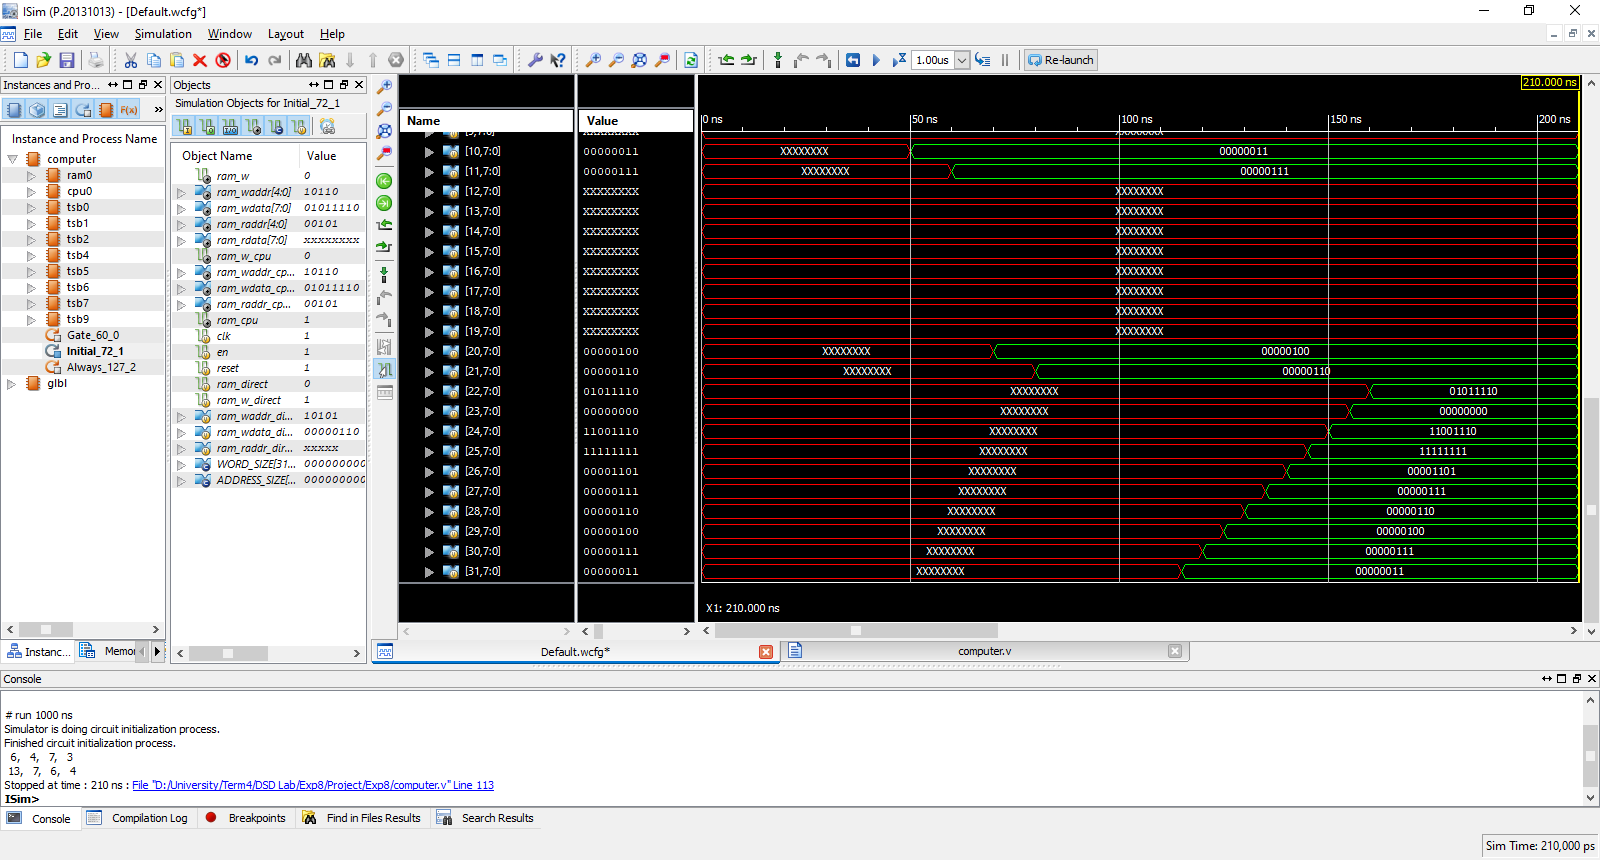
\includegraphics[width=\linewidth]{mem.png}
	\caption{حاصل شبیه‌سازی \lr{computer.v}}
\end{figure}

\end{document}
